\documentclass{beamer}
\usepackage{progressbar, tcolorbox, CJKutf8, hyperref, multicol, pdfpages, graphicx, xcolor, blindtext, tikz, pgfplots}
\usepackage[absolute,overlay]{textpos}
\usepackage[backend=bibtex,style=numeric,sorting=none]{biblatex}

\hypersetup{
    colorlinks=true,
    linkcolor=blue,
    filecolor=magenta,      
    urlcolor=blue,
    }

\graphicspath{ {./images/} }
\usetheme{AnnArbor}
\addbibresource{main.bib}
\usetikzlibrary{positioning, calc, shapes.multipart, shapes.arrows, fit, backgrounds}

\definecolor{dockerColor}{RGB}{13, 183, 237}
\definecolor{secureColor}{RGB}{10, 191, 83}
\definecolor{aquamarine}{rgb}{0.5, 1.0, 0.83}
\definecolor{aquamarine2}{rgb}{0.2, 1.0, 0.53}

\title{The Container Security in Healthcare Data Exchange System}
\subtitle{Bachelor's degree graduation project}
\author{Chih-Hsuan Yang}
\institute{National Sun Yat-sen University\\
Advisor: Chun-I Fan
}
\date{\today}

\AtBeginSection[]{
  \begin{frame}
  \vfill
  \centering
  \begin{beamercolorbox}[sep=8pt,center,shadow=true,rounded=true]{title}
    \usebeamerfont{title}\insertsectionhead\par%
  \end{beamercolorbox}
  \vfill
  \end{frame}
}



\begin{document}
\begin{CJK*}{UTF8}{bsmi}

  \begin{frame}
    \titlepage
  \end{frame}


  \begin{frame}{Outline}
    \begin{multicols}{2}
      \tableofcontents
    \end{multicols}
  \end{frame}

  \section{Attack}
  \begin{frame}{Attacking surfaces}
    \begin{itemize}
      \item Escape: runC, kernel exploit
      \item malicious images
      \item inner-container app's attack
    \end{itemize}
  \end{frame}

  \section{Defense}
  \begin{frame}{The runC and the kernel exploit}
    The kernel exploit is not considered in this project.\\
    The runC vulnerability will be discussed later.
  \end{frame}

  \begin{frame}{Images and containers(runtime)}
    Sign it. (The whole digital signature)\\
    Scan it. (Recursively brute force to scan the file system, just like the anti-virus)
  \end{frame}

  \begin{frame}{Inner-container protection}
    \begin{itemize}
      \item Configuration-based: Just like the Cilium and docker arguments
      \item Code-based: Seccomp, LSM
      \item {\color{green} Rule-based}: Rules in Apparmor, SELinux...
    \end{itemize}
    Well\dots\\
    Some papers... \cite*{217614, Gao2017ContainerLeaksES, Access_Control_Architecture}
  \end{frame}

  \begin{frame}{I don't want}
    Make the fourth way: AI-based\\
    Use the CNN, DNN or some AI algorithms.
  \end{frame}

  \begin{frame}{The runC: CVE-2019-5736}

    \begin{multicols*}{2}
      \begin{beamerboxesrounded}[width=.5\textwidth]{\href{https://github.com/Frichetten/CVE-2019-5736-PoC/blob/master/main.go}{PoC}}
        \begin{itemize}
          \item Must run in the privileged container.
          \item Try to overwrite the /sbin/init program, a.k.a the runC program's binary file.
          \item Busy waiting to overwrite.
        \end{itemize}
      \end{beamerboxesrounded}

      \begin{beamerboxesrounded}[width=.5\textwidth]{\href{https://github.com/lxc/lxc/commit/6400238d08cdf1ca20d49bafb85f4e224348bf9d}{Patch}}
        \begin{itemize}
          \item Create a temporary copy of the calling binary itself when it starts.
          \item Using the memfd\_create() system call and copies itself into the temporary in-memory file.
          \item Execute this memfd.
          \item Redirect the write operations from a privileged container to the in-memory binary.
          \item However, the in-memory binary is sealed, writes to this will also fail.
        \end{itemize}
      \end{beamerboxesrounded}
    \end{multicols*}

  \end{frame}

  \begin{frame}
    \centering
    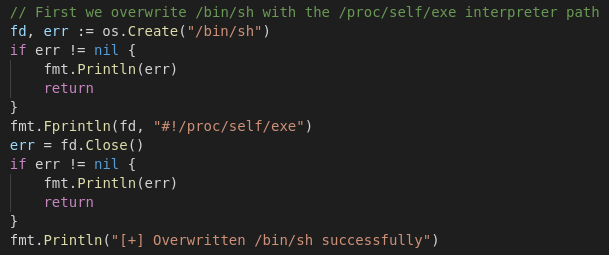
\includegraphics[width=.7\textwidth]{runc1.png}
    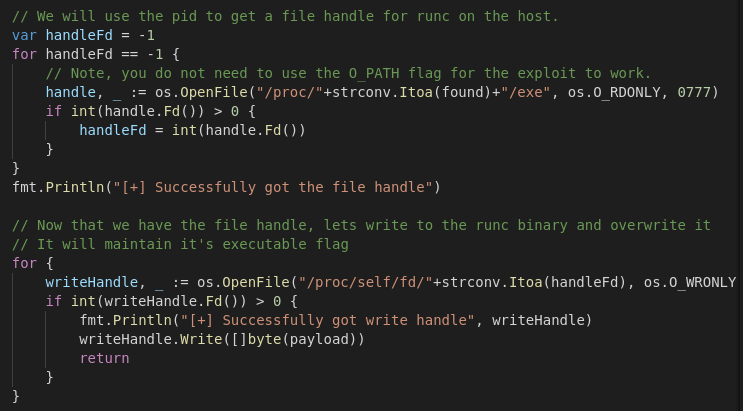
\includegraphics[width=.7\textwidth]{runc2.png}
  \end{frame}

  \begin{frame}
    \centering
    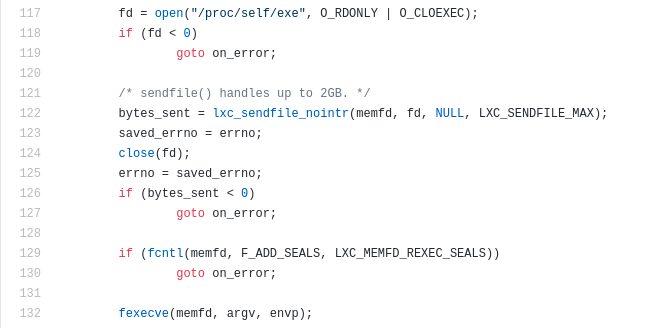
\includegraphics[width=\textwidth]{rexec.png}
  \end{frame}

  \section{Planing}
  \begin{frame}{Discuss with senior and Tim Hsu}
    \centering
    
\includegraphics[width=\textwidth]{Screenshot_2021-07-16_03-14-43.png}
    Give me one more week \dots\\
    I know the summer is not so long.
  \end{frame}

  \begin{frame}{References}
    \def\bibfont{\footnotesize}
    \printbibliography
  \end{frame}

\end{CJK*}
\end{document}